% Capítulo 5: árvore da expressão (3 + 5) * 4 - 2, com os termos principais.
\documentclass[border=4pt]{standalone}
\usepackage[utf8]{inputenc}
\usepackage[T1]{fontenc}
% Estilo comum das figuras de árvores (capítulo 5).
\usepackage{tikz}
\usetikzlibrary{arrows.meta, positioning, calc}
\definecolor{navy}{RGB}{23,45,80}
\definecolor{laranja}{RGB}{250,110,29}
\definecolor{cinzalogo}{RGB}{107,114,126}
\tikzset{
  vertice/.style={circle, draw=navy, line width=0.9pt, fill=laranja!12, minimum size=8mm,
                  inner sep=0pt, font=\sffamily\small},
  destaque/.style={vertice, fill=laranja!45, draw=laranja},
  apagado/.style={vertice, dashed, draw=cinzalogo, fill=white, text=cinzalogo},
  arvore/.style={level distance=12mm, edge from parent/.style={draw=navy, line width=0.9pt}},
  rotulo/.style={font=\sffamily\small\bfseries, text=navy},
  legenda/.style={font=\sffamily\scriptsize, text=cinzalogo},
  setanova/.style={-{Stealth[length=2.2mm]}, laranja, line width=1.3pt},
}

\begin{document}
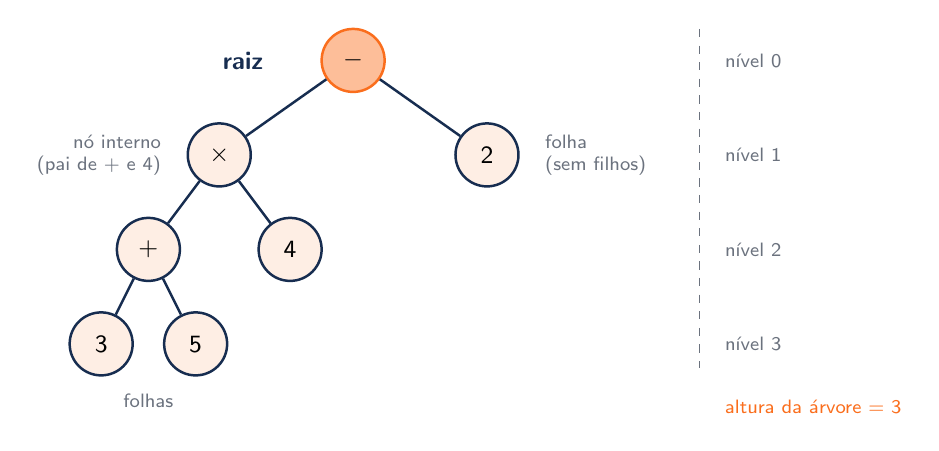
\begin{tikzpicture}[arvore, level 1/.style={sibling distance=34mm}, level 2/.style={sibling distance=18mm},
                    level 3/.style={sibling distance=12mm}]
  \node[destaque] (raiz) {$-$}
    child {node[vertice] (mult) {$\times$}
      child {node[vertice] (mais) {$+$}
        child {node[vertice] (tres) {3}}
        child {node[vertice] (cinco) {5}}}
      child {node[vertice] (quatro) {4}}}
    child {node[vertice] (dois) {2}};
  % rótulos
  \node[rotulo, left=6mm of raiz] {raiz};
  \node[legenda, right=2mm of dois, align=left] {folha\\(sem filhos)};
  \node[legenda, below=1mm of tres, xshift=6mm] {folhas};
  \node[legenda, left=2mm of mult, align=right] {nó interno\\(pai de + e 4)};
  % níveis
  \foreach \y/\n in {0/0, -1.2/1, -2.4/2, -3.6/3} {
    \node[legenda, anchor=west] at (4.6,\y) {nível \n};
  }
  \draw[cinzalogo, dashed] (4.4,0.4) -- (4.4,-3.9);
  \node[legenda, anchor=west, text=laranja] at (4.6,-4.4) {altura da árvore = 3};
\end{tikzpicture}
\end{document}
